\documentclass[11pt]{beamer}
\usetheme{Madrid}
\usefonttheme{serif}

\usepackage[utf8]{inputenc}
\usepackage[english]{babel}
\usepackage[T1]{fontenc}

\usepackage{amsmath}
\usepackage{amsfonts}
\usepackage{amssymb}
\usepackage{graphicx}

\setbeamertemplate{caption}[numbered]
\setbeamertemplate{navigation symbols}{}

% Author / Title Info
% Author / Title Info
\author[Team]{%
\begin{tabular}{lll}
Goureesh Chandra   & 31 & TVE22CS069 \\
Ivin Mathew Kurian & 33 & TVE22CS075 \\
Muhammed Farhan    & 39 & TVE22CS094 \\
Rethin Francis     & 72 & LTVE22CS149 \\
\end{tabular} \\[8pt]
\textbf{Advisor: Prof. Divya S K}
}

\title{Reinforcement Learning for ICU Treatment Planning}

\institute[]{College of Engineering, Trivandrum \\ Dept. of Computer Science \& Engineering}
\date{\today}

% ---------------------------------------------------------
\begin{document}

% Title
\begin{frame}
  \titlepage
\end{frame}

% Table of Contents
\begin{frame}{Contents}
  \tableofcontents
\end{frame}




% --------------------------------------
\section{Introduction}
\begin{frame}{Introduction}
Doctors often face tough choices when treating critically ill patients.  
\vspace{6pt}

Our project builds an \textbf{AI system} that learns from hospital data to suggest better treatment plans.  
\vspace{6pt}

The goal is to support doctors, make care safer, and improve patient outcomes.  
\end{frame}


% --------------------------------------
\section{Problem Statement}
\begin{frame}{Problem Statement}
Making timely and personalized treatment decisions for patients with complex, evolving conditions is a significant clinical challenge.

\begin{itemize}
    \item \textbf{High-Stakes Decisions} – Clinicians must manage highly dynamic patient trajectories where standardized protocols are often insufficient.
    \item \textbf{Fragmented Data} – Patient health records are often scattered and incomplete, hindering a comprehensive view for effective treatment.
    \item \textbf{Learning Constraints} – Existing AI methods are often limited to mimicking historical data and cannot safely explore potentially better treatment strategies.
\end{itemize}
\end{frame}

% --------------------------------------
\section{Objective}
\begin{frame}{Objective}
The objective of this project is to develop a novel AI framework using model-based reinforcement learning to provide personalized and safer clinical decision support.

\begin{itemize}
    \item \textbf{Patient Simulator ("Digital Twin")} – Learn and simulate patient physiological dynamics from historical clinical data.
    \item \textbf{AI-Driven Policy Optimization} – Use the simulator as a safe environment to train a reinforcement learning agent to discover optimal and personalized treatment strategies.
    \item \textbf{Clinical Decision Support} – Deliver data-driven treatment recommendations to support clinicians, improve patient outcomes, and enhance safety.
\end{itemize}
\end{frame}



% --------------------------------------
\section{Literature Review}

% Slide 1
\begin{frame}[t]{Literature Review}
\small
\resizebox{\textwidth}{!}{%
\begin{tabular}{|p{1cm}|p{4cm}|p{3cm}|p{4cm}|p{2.5cm}|p{5cm}|}
\hline
\textbf{Sl. no.} & \textbf{Name of Publication} & \textbf{Journal / Conference} & \textbf{Author(s)} & \textbf{Date of publication} & \textbf{Remarks} \\
\hline
1 & \textbf{Challenges with reinforcement learning model transportability for sepsis treatment in emergency care} & Critical Care Medicine & A. Komorowski et al. & 2021 & \textbf{Advantage:} Explores transportability of RL models from ICU to ED, addressing real-world sepsis care needs. \newline \textbf{Disadvantage:} ICU-trained models struggle due to missing ED data, limiting applicability. \\
\hline
2 & \textbf{Deep learning prediction models based on EHR trajectories: A systematic review} & Journal of Biomedical Informatics & Ali Amirahmadi, Mattias Ohlsson, and Kobra Etminani & 2023 & \textbf{Advantage:} Provides comprehensive review of deep learning for EHR trajectory prediction, highlighting RNNs and attention. \newline \textbf{Disadvantage:} Challenges include data insufficiency, explainability, and handling complex dependencies. \\
\hline
3 & \textbf{Deep offline reinforcement learning for real-world treatment optimization applications} & arXiv Preprint & Mila Nambiar et al. & 2023 & \textbf{Advantage:} Introduces transition sampling to improve offline RL, achieving better safety and constraint satisfaction in sepsis/diabetes. \newline \textbf{Disadvantage:} Offline RL limited by suboptimal retrospective data and strict safety needs. \\
\hline
4 & \textbf{Learning transformer based world models with contrastive predictive coding} & NeurIPS & Anon. Authors & 2021 & \textbf{Advantage:} TWISTER achieves SOTA on Atari 100k without search, showing the power of contrastive objectives in Transformers. \newline \textbf{Disadvantage:} Prior Transformer models underperform due to weak next-state objectives. \\
\hline
\end{tabular}}
\end{frame}

% Slide 2
\begin{frame}[t]{Literature Review (contd.)}
\small
\resizebox{\textwidth}{!}{%
\begin{tabular}{|p{1cm}|p{4cm}|p{3cm}|p{4cm}|p{2.5cm}|p{5cm}|}
\hline
\textbf{Sl. no.} & \textbf{Name of Publication} & \textbf{Journal / Conference} & \textbf{Author(s)} & \textbf{Date of publication} & \textbf{Remarks} \\
\hline
5 & \textbf{Mastering Memory Tasks with World Models} & ICML & Anon. Authors & 2023 & \textbf{Advantage:} R2I enables state-of-the-art memory/credit assignment, outperforming DreamerV3 in BSuite and POPGym. \newline \textbf{Disadvantage:} MBRL agents still struggle with long-term dependencies and recalling distant observations. \\
\hline
6 & \textbf{Predicting the impact of treatments over time with uncertainty aware neural differential equations} & AISTATS & Edward De Brouwer, Javier González Hernández, and Stephanie Hyland & 2022 & \textbf{Advantage:} CF-ODE provides accurate treatment impact predictions with uncertainty estimates. \newline \textbf{Disadvantage:} Counterfactual prediction limited due to confounding in observational data. \\
\hline
7 & \textbf{Reinforcement Learning in Healthcare - Optimizing treatment strategies dynamic resource allocation and adaptive clinical decision making} & Int. J. of Computer Applications Tech. & Hassan Ali & 2022 & \textbf{Advantage:} Broad survey of RL in healthcare, covering treatment optimization, resource allocation, and adaptive decision-making. \newline \textbf{Disadvantage:} Does not provide detailed shortcomings since it is a review, not an experiment. \\
\hline
8 & \textbf{Safe Reinforcement Learning for Sepsis Treatment} & IEEE Int. Conf. on Healthcare Informatics & Yan Jia et al. & 2020 & \textbf{Advantage:} Introduces safe RL approaches for sepsis care, with focus on safety constraints. \newline \textbf{Disadvantage:} Early-stage proceedings paper, lacks in-depth limitation analysis. \\
\hline
\end{tabular}}
\end{frame}

% Slide 3
\begin{frame}[t]{Literature Review (contd.)}
\small
\resizebox{\textwidth}{!}{%
\begin{tabular}{|p{1cm}|p{4cm}|p{3cm}|p{4cm}|p{2.5cm}|p{5cm}|}
\hline
\textbf{Sl. no.} & \textbf{Name of Publication} & \textbf{Journal / Conference} & \textbf{Author(s)} & \textbf{Date of publication} & \textbf{Remarks} \\
\hline
9 & \textbf{Smart Imitator: Learning from Imperfect Clinical Decisions} & arXiv Preprint & Anon. Authors & 2021 & \textbf{Advantage:} Combines imitation learning with RL to learn from imperfect clinical data, outperforming baselines on sepsis/diabetes. \newline \textbf{Disadvantage:} Struggles with high-risk patient treatment due to data scarcity. \\
\hline
10 & \textbf{Towards Safe Mechanical Ventilation Treatment Using Deep Offline Reinforcement Learning} & AAAI-23 & Flemming Kondrup et al. & 2023 & \textbf{Advantage:} Proposes DeepVent, a CQL-based safe offline DRL agent, optimizing ventilation parameters for 90-day survival. \newline \textbf{Disadvantage:} Explicit limitations not detailed, focus mainly on safety improvements. \\
\hline
\end{tabular}}
\end{frame}

%---------------------------------------
\section{Research Gaps}
\begin{frame}{Research Gaps}
\begin{itemize}
    \item \textbf{Incomplete and irregular EHR data} – missing values, noise, and inconsistent sampling limit effective learning.
    \vspace{6pt}
    \item \textbf{Over-reliance on offline RL} – many systems copy historical clinician decisions instead of exploring new strategies.
    \vspace{6pt}
    \item \textbf{Limited patient personalization} – existing models often treat all patients similarly, ignoring individual differences.
    \vspace{6pt}
    \item \textbf{Safety concerns in real-world testing} – direct deployment on patients is risky without reliable simulators.
    \vspace{6pt}
    \item \textbf{Generalization challenges} – models trained on one dataset (e.g., MIMIC) may not transfer well to other hospitals.
\end{itemize}
\end{frame}



% --------------------------------------
\section{Proposed Solution Methodology}
\begin{frame}{Proposed Solution Methodology}
This approach is inspired by DreamerV3 and its clinical adaptation in medDreamer.  

\textbf{Two sequential stages:}
\begin{enumerate}
    \item Train the \textbf{Patient Simulator (World Model)} to predict patient outcomes.  
    \item Train the \textbf{RL Agent (Policy)} using the simulator to discover optimal treatments.
\end{enumerate}
\end{frame}

% ------------------------------------------------------
\begin{frame}{Algorithm 1: Patient Simulator Training}
\textbf{Goal:} Learn patient health dynamics from EHR data to create a reliable "digital twin".  

\textbf{Steps:}
\begin{enumerate}
    \item \textbf{Initialization:} Neural network parameters $\phi$  
    \begin{itemize}
        \item Encoder
        \item Dynamics predictor
        \item Prediction heads (reconstruction, rewards, outcomes)
    \end{itemize}
    \item \textbf{Training Loop:} For multiple epochs:
    \begin{enumerate}
        \item Sample patient trajectories (observations, actions, rewards)
        \item Encode observations to latent states $s_t$
        \item Predict next latent state $s_{t+1}$ given $s_t$ and action $a_t$
        \item Reconstruct observations and predict rewards/outcomes
        \item Compute combined loss and update $\phi$ via backpropagation
    \end{enumerate}
    \item \textbf{Output:} Trained Patient Simulator for realistic patient trajectories
\end{enumerate}
\end{frame}

% ------------------------------------------------------
\begin{frame}{Algorithm 2: RL Agent Training}
\textbf{Goal:} Train an optimal treatment policy safely in the simulated environment.

\textbf{Steps:}
\begin{enumerate}
    \item Load trained Patient Simulator (weights frozen)
    \item Initialize RL Agent: policy network $\theta$ (actor), value network $\psi$ (critic)
\end{enumerate}

\textbf{Phase 1: Clinically Grounded Policy Initialization}  
\begin{itemize}
    \item Generate hybrid trajectories (real data + short simulator rollouts)
    \item Train actor and critic:
    \begin{itemize}
        \item Critic: evaluate long-term state values
        \item Actor: choose actions leading to high-value states
    \end{itemize}
\end{itemize}
\end{frame}

% ------------------------------------------------------
\begin{frame}{Algorithm 2 (cont.): Strategic Refinement}
\textbf{Phase 2: Strategic Refinement through Long-Horizon Imagination}  
\begin{itemize}
    \item Generate fully imagined trajectories using the Patient Simulator
    \item Fine-tune actor and critic to improve long-term planning
\end{itemize}

\textbf{Output:} Final trained \textbf{Optimal Treatment Policy} that recommends actions given a patient’s current state
\end{frame}

%--------------------------------------------------------
\section{Design of Proposed Methodology}
\begin{frame}{Design of Proposed Methodology}
    \begin{center}
        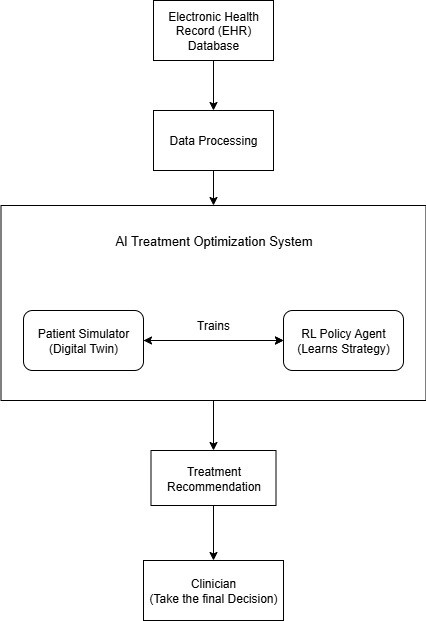
\includegraphics[width=0.45\textwidth]{design_flow.jpg} % Replace with your image file
    \end{center}
\end{frame}

\begin{frame}{Design Flow (Contd.)}
    \textbf{1. Electronic Health Record (EHR) Database}
    \begin{itemize}
        \item Large, de-identified patient records (vitals, labs, diagnoses, meds)
        \item Source of "experience" for the AI
        \item Example: MIMIC-IV
    \end{itemize}

    \vspace{0.3cm}
    \textbf{2. Data Preprocessing}
    \begin{itemize}
        \item Clean and structure messy clinical data
        \item Handle missing/irregular data
        \item Convert into patient timelines/trajectories
    \end{itemize}
\end{frame}

\begin{frame}{Design Flow (Contd.)}
    \textbf{3A. Patient Simulator ("Digital Twin")}
    \begin{itemize}
        \item Model predicts patient response to treatments
        \item Provides safe virtual testing ground
        \item Based on model-based RL (e.g., DreamerV3)
    \end{itemize}

    \vspace{0.3cm}
    \textbf{3B. RL Policy Agent}
    \begin{itemize}
        \item Learns best actions through trial-and-error in simulator
        \item Maps patient state → treatment decision
        \item Optimizes for long-term stability/survival
    \end{itemize}
\end{frame}

\begin{frame}{Design Flow (Contd.)}
    \textbf{4. Treatment Recommendation}
    \begin{itemize}
        \item AI suggests adaptive treatment actions (e.g., dosage)
        \item Produces a Dynamic Treatment Regime (DTR)
    \end{itemize}

    \vspace{0.3cm}
    \textbf{5. Clinician (Final Decision)}
    \begin{itemize}
        \item Doctor reviews AI suggestions
        \item Combines with expertise, ethics, patient context
        \item Ensures safety and accountability
    \end{itemize}
\end{frame}

% --------------------------------------
\section{Resource Allocation}
\begin{frame}{Resource Allocation}
\textbf{1. Data Resources}  
\begin{itemize}
    \item MIMIC-III, MIMIC-IV, eICU datasets.
    \item Preprocessing: Python (pandas, NumPy, scikit-learn).
\end{itemize}

\textbf{2. Computational Resources}  
\begin{itemize}
    \item GPU-enabled system (RTX 4060/4090 or cloud GPUs).
    \item Frameworks: PyTorch, Ray RLlib.
\end{itemize}
\end{frame}



% --------------------------------------
\section{Future Work}
\begin{frame}{Future Work}
\begin{itemize}
    \item Extend framework to other diseases (e.g., diabetes, cancer care).  
    \item Incorporate multi-modal data (genomics, imaging).  
    \item Clinician-in-the-loop evaluation.  
\end{itemize}
\end{frame}


% --------------------------------------
\section{Conclusion}
\begin{frame}{Conclusion}
\begin{itemize}
    \item We are developing a \textbf{model-based reinforcement learning framework} trained on ICU data for clinical decision support.  
    \vspace{6pt}
    \item By building a \textbf{digital twin of patients}, the system safely explores treatment strategies without direct risk to patients.  
    \vspace{6pt}
    \item The approach enables \textbf{personalized and safer treatment recommendations}, reducing unnecessary interventions and improving patient outcomes.  
    \vspace{6pt}
    \item Future work includes extending the model to more diverse patient populations and validating in real-world clinical settings.  
\end{itemize}
\end{frame}



% --------------------------------------
\section{References}
\begin{frame}{References}
\tiny
\begin{thebibliography}{9}

\bibitem{xu2025}
Qianyi Xu, Dilruk Perera, Gousia Habib, and Mengling Feng (2025).
\newblock medDreamer: Model-Based Reinforcement Learning with Latent Imagination on Complex EHRs for Clinical Decision Support.
\newblock \textit{arXiv preprint arXiv:2505.19785}.

\bibitem{komorowski2021}
Arthur Komorowski et al. (2021).
\newblock Challenges with reinforcement learning model transportability for sepsis treatment in emergency care.
\newblock \textit{Critical Care Medicine}.

\bibitem{amirahmadi2023}
Ali Amirahmadi, Mattias Ohlsson, and Kobra Etminani (2023).
\newblock Deep learning prediction models based on EHR trajectories: A systematic review.
\newblock \textit{Journal of Biomedical Informatics}.

\bibitem{nambiar2023}
Mila Nambiar et al. (2023).
\newblock Deep offline reinforcement learning for real-world treatment optimization applications.
\newblock \textit{arXiv preprint arXiv:2302.07549}.


\bibitem{r2i2023}
Anon. Authors (2023).
\newblock Mastering Memory Tasks with World Models.
\newblock \textit{ICML}.

\bibitem{debrouwer2022}
Edward De Brouwer, Javier González Hernández, and Stephanie Hyland (2022).
\newblock Predicting the impact of treatments over time with uncertainty aware neural differential equations.
\newblock \textit{AISTATS}.

\bibitem{kondrup2023}
Flemming Kondrup et al. (2023).
\newblock Towards Safe Mechanical Ventilation Treatment Using Deep Offline Reinforcement Learning.
\newblock \textit{AAAI-23}.

\end{thebibliography}
\end{frame}


% --------------------------------------
\begin{frame}
\begin{center}
    \Huge{Thank You!}
\end{center}
\end{frame}

\end{document}
